\documentclass[11pt,a4paper]{article}
\usepackage[T1]{fontenc}
\usepackage[utf8]{inputenc}
\usepackage[margin=2.3cm,top=2.1cm,bottom=2.0cm]{geometry}
\usepackage{lmodern}
\usepackage{microtype}
\usepackage{xcolor}
\usepackage{enumitem}
\usepackage{titlesec}
\usepackage{tcolorbox}
\usepackage{tikz}
\usepackage[hidelinks]{hyperref}
\usetikzlibrary{positioning,arrows.meta}

\definecolor{ink}{HTML}{16201B}
\definecolor{accent}{HTML}{1A6B3C}
\definecolor{muted}{HTML}{5D6B64}
\definecolor{rule}{HTML}{D7DED9}
\definecolor{soft}{HTML}{F4F7F5}

\color{ink}
\titleformat{\section}{\large\bfseries\color{accent}}{}{0em}{}
\titlespacing*{\section}{0pt}{12pt}{4pt}
\setlist[itemize]{leftmargin=1.1em,itemsep=2.5pt,topsep=3pt}
\setlength{\parskip}{4pt}
\setlength{\parindent}{0pt}
\pagestyle{empty}

\newtcolorbox{keybox}{colback=soft,colframe=rule,boxrule=0.6pt,
  arc=2pt,left=8pt,right=8pt,top=6pt,bottom=6pt}

\begin{document}

\noindent{\Huge\bfseries\color{accent} ReqShift}\par
\vspace{3pt}
\noindent{\large\color{muted} Requirements prose in, a proved goal model out.}\par
\vspace{6pt}
\noindent\textcolor{rule}{\rule{\linewidth}{1pt}}

\section{What it is}

ReqShift reads an engineering requirements document written in ordinary language and
turns it into a model a solver can reason about. It then reports what the solver
proved about that model.

It is built on top of GoalShift, the analysis tool behind the thesis. GoalShift does
the proving. ReqShift is the front end that gets a real document into a form GoalShift
can accept, which until now had to be done by hand.

\section{The problem it addresses}

Modern machines are rarely one machine. A line has a variable number of robots. A
warehouse has a variable number of shuttles. A charging site has a variable number of
chargers and vehicles.

Requirements documents almost never say how many. They describe what each part must
do, and they leave the question of how many of each part will actually be present to
be settled later, on site. Nobody checks whether the system still works at every
combination the document allows.

\begin{keybox}
A study of 31 real requirements documents across four industries found the same thing
every time. The documents state the behaviour. They do not state the composition. The
gap is not an oversight in one document. It is how these documents are written.
\end{keybox}

\section{What it does, in four steps}

\begin{center}
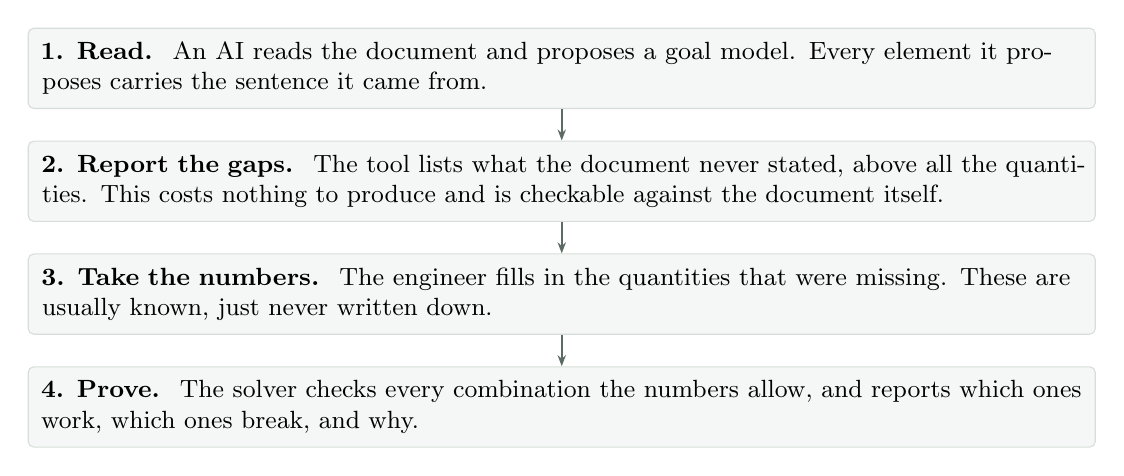
\begin{tikzpicture}[
  node distance=4mm,
  box/.style={draw=rule,fill=soft,rounded corners=2pt,inner sep=5pt,
              text width=13.2cm,align=left,font=\small},
  arr/.style={-{Stealth[length=4pt]},draw=muted,thick}]

\node[box] (a) {\textbf{1. Read.}\; An AI reads the document and proposes a goal
  model. Every element it proposes carries the sentence it came from.};
\node[box,below=of a] (b) {\textbf{2. Report the gaps.}\; The tool lists what the
  document never stated, above all the quantities. This costs nothing to produce and
  is checkable against the document itself.};
\node[box,below=of b] (c) {\textbf{3. Take the numbers.}\; The engineer fills in the
  quantities that were missing. These are usually known, just never written down.};
\node[box,below=of c] (d) {\textbf{4. Prove.}\; The solver checks every combination
  the numbers allow, and reports which ones work, which ones break, and why.};

\draw[arr] (a) -- (b);
\draw[arr] (b) -- (c);
\draw[arr] (c) -- (d);
\end{tikzpicture}
\end{center}

\section{What comes out}

The solver does not return an opinion. It returns facts about the model, and each one
traces back to a sentence in the document.

\begin{itemize}
  \item \textbf{Behaviour classes.} Out of all the combinations the document permits,
    only a handful behave differently from each other. The tool finds that handful.
    Twenty four possible configurations often collapse to four distinct behaviours.
  \item \textbf{Broken configurations.} The exact combinations in which some part of
    the system cannot meet its goal, named one by one.
  \item \textbf{Numbers that do nothing.} Upper limits written into the document that
    cannot change any outcome. These can be shown to be decoration rather than
    guessed at.
  \item \textbf{Real ceilings.} Where one part limits another. For example a fleet
    capped at seven by the capacity of what serves it, not by its own stated maximum
    of twelve.
\end{itemize}

\section{Why the answers can be trusted}

This is the part that matters most, so it is worth being precise about it.

A language model cannot tell you when it is wrong. A solver cannot read prose. Their
weaknesses are opposites, so each one covers the other. ReqShift uses each for only
the job it is good at.

\begin{keybox}
\textbf{The AI produces the input. The solver produces the answer.}

The AI writes a draft goal model, which a person reviews. Every finding after that
point is computed arithmetically from the solver's output, by code that never calls a
language model at all. A finding cannot be invented, because nothing that invents
things is involved in producing it.
\end{keybox}

The draft is meant to be reviewed, not trusted. That is why every element the AI
proposes is shown next to the sentence it was taken from, and why the tool separates
what the document actually stated from what the AI assumed.

\section{What it does not do}

\begin{itemize}
  \item It does not check that the requirements are the right requirements. It checks
    that they hold together, and that the system works at every permitted size.
  \item It does not replace the engineer's review of the model. The AI drafts, a
    person confirms.
  \item It cannot find something the document never mentioned. If a whole part of the
    system is missing from the text, it is missing from the model.
  \item It applies to systems with a variable number of parts. For a single fixed
    machine there is nothing for it to say.
\end{itemize}

\section{Where it stands today}

The analysis engine is the one described in the thesis and it is finished. It has been
run end to end on real requirements documents from four different industries, and on a
hand built case study which it reproduced from the text alone.

There are two engines behind it. The default is the SAT engine from the thesis, whose
results are proved by the published encoding. A second, experimental engine based on
z3 handles larger quantities and can also take timing and capacity into account. The
two agree on every model both can express, checked over seventy seven generated test
models with no disagreement.

\vspace{12pt}
\noindent\textcolor{rule}{\rule{\linewidth}{0.6pt}}
\vspace{2pt}

{\footnotesize\color{muted}
GoalShift is the analysis tool described in the thesis and is not modified by ReqShift.
It is imported unchanged, so the artifact the research describes stays exactly as it
was.}

\end{document}
